\begin{frame}
    \frametitle{Introduction à OpenCL}  

    Couche d'abstraction matériel: cibler GPU, CPU et FPGA\pause{}
    \vspace{10pt}

    Programme hôte (Python)\pause{}

    Kernels:\pause{}
    \begin{itemize}
        \item Dérivé du C99\pause{}
        \item Fonctionnalités enlevées:\pause{}
            \begin{itemize}
                \item Récursivité
                \item Pointeurs de fonctions
                \item Allocation dynamique
                \item \textit{bit fields}
            \end{itemize}\pause{}
        \item Fonctionnalités ajoutées:\pause{}
            \begin{itemize}
                \item Types spéciaux e.g. \textit{float4}
                \item Fonctions spéciales e.g. \textit{barrier}
            \end{itemize}
    \end{itemize}\pause{}
    \vspace{10pt}

    Opérations sont des événements

    Opérations placées dans une file d'exécution: \textit{queue}\pause{}
    \vspace{10pt}

    Plusieurs modèles à comprendre:\pause{}
    \begin{itemize}
        \item modèle d'exécution
        \item modèle de mémoire
    \end{itemize}
\end{frame}

\begin{frame}
    \frametitle{Modèle d'exécution}

    \textit{NDRange}: \textit{N-dimensions range}\pause{}
    \begin{itemize}
        \item \textit{Global NDRange}: G
        \item \textit{Local NDRange}: L
    \end{itemize}\pause{}
    
    Au lancement d'un Kernel:
    \begin{itemize}
        \item \textit{work item}:\pause{} 
            \begin{itemize}
                \item ${\displaystyle nombre(\textrm{work items}) = \prod_{i=0}^{N}G[i]}$\pause{}
                \item exécute le kernel
                \item exécution concurrente
            \end{itemize}

        \item \textit{work group}:\pause{}
            \begin{itemize}
                \item regroupe les \textit{work items}\pause{}
                \item ${\displaystyle nombre(\textrm{work groups}) = nombre(\textrm{work items}) /
                    \prod_{i=0}^{N}L[i]}$\pause{}
                \item exécution parallèle
                \item exécuté par les \textit{compute units}
            \end{itemize}
    \end{itemize}
\end{frame}

\begin{frame}
    \frametitle{Modèle d'exécution}
    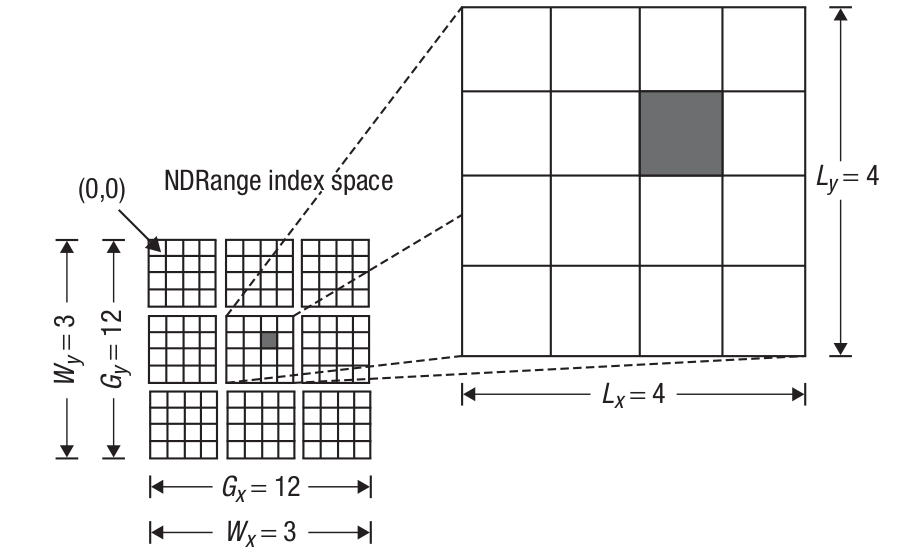
\includegraphics[width=\textwidth]{../resources/execution_model.png}
\end{frame}

\begin{frame}
    \frametitle{Modèle de mémoire}
    \textit{Memory objects}:\pause{}
    \begin{itemize}
        \item \textit{buffer objects}
        \item \textit{image objects}
    \end{itemize}\pause{}
    \vspace{20pt}

    5 régions de mémoire:\pause{}
    \begin{itemize}
        \item \textit{host memory}: accessible uniquement par l'hôte\pause{}
        \item \textit{global memory}: accessible par tous\pause{}
        \item \textit{constant memory}: comme la mémoire globale mais constante\pause{}
        \item \textit{local memory}: lié à un \textit{work group}\pause{}
        \item \textit{private memory}: lié à un \textit{work item}
    \end{itemize}
\end{frame}

\begin{frame}
    \frametitle{Modèle de mémoire}
    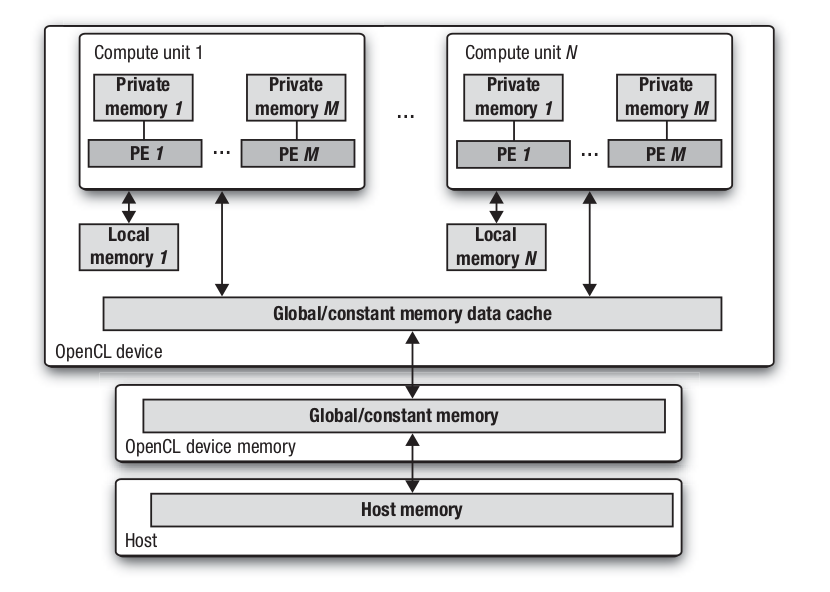
\includegraphics[width=\textwidth]{../resources/memory_model.png}
\end{frame}
